\documentclass[11pt]{article}
\usepackage[utf8]{inputenc}
\usepackage{amssymb,amsmath,amsthm,mathtools}
\usepackage[english]{babel}

\newtheorem{theorem}{Theorem}[section]
\newtheorem{corollary}{Corollary}[theorem]
\newtheorem{lemma}[theorem]{Lemma}

\topmargin -0.5in
\textheight 9.0in
\oddsidemargin  -0.05in
\evensidemargin -0.05in
\textwidth 6.5in
\renewcommand
\baselinestretch{1.0}

\newcommand{\tr}{{\text{tr}}}
\newcommand{\B}[1]{\textbf{#1}}
\newcommand{\T}[1]{\texttt{#1}}

\title{The Qudit Arthurs-Kelly Measurement}
\author{Matthew B. Weiss}

\begin{document}
\maketitle

\section{Introduction}

In 1965, Arthurs and Kelly \cite{ArthursKelly, PhysRevA.43.1153} proposed a realization of the canonical coherent state measurement using the following scheme. Two ancilla systems begin in Gaussian states centered at the origin of the infinite line; the ancillas are then coupled to a system of interest such that system's position drives translations of the first ancilla, and the system's momentum drives translations of the second ancilla. Upon position measurements of the two ancillas, by analyzing the resulting Kraus operators, it is possible to show that one ought to project the system state into a coherent state with the appropriate probability. Recall that the coherent states may be obtained as the orbit of the vacuum state under the Weyl-Heisenberg (WH) group. In fact, the Arthurs-Kelly procedure may realize more general WH-covariant measurements for different choices of initial states for the ancillas.

 In this note, we show how the Arthurs-Kelly measurement may be adapted to finite dimensional systems, or qudits. In the case that $d=2^n$, we provide a recipe for decomposing the required qudit operations into one and two qubit operations. One special class of finite-dimensional WH-covariant measurements are SIC-POVMs (symmetric informationally-complete) \cite{Renes_2004}: a SIC's $d^2$ rank-1 POVM elements may be rescaled into pure states which form a regular simplex inscribed in quantum state-space, and in all save one sporadic case, SICs are covariant under the discrete WH group \cite{Stacey2021}. We specialize to the implementation of a  SIC in dimension four.

\section{Weyl-Heisenberg operators}

Fixing a Hilbert space $\mathcal{H}_d$, let clock and shift operators \cite{Gross_2021} be defined as
\begin{align}
Z|m\rangle = \omega^{m}|m\rangle && 	X|m\rangle = |m+1\rangle
\end{align}
where $\{|m\rangle\}_{m=0}^{d-1}$ denote  discrete position states (which we may take to be the computational basis states) and $\omega=e^{2\pi i/d}$. Note that all addition is understood mod $d$. The clock and shift  operators satisfy the relation $ZX=\omega XZ$, and we may use them to define a representation (up to phase) of the group $\mathbb{Z}_d\times \mathbb{Z}_d$ in terms of Weyl-Heisenberg (WH) displacement operators
\begin{align}
D_{\B{a}}=X^{a_1}Z^{a_2} && \B{a}=(a_1, a_2)\in \mathbb{Z}_{d}^2.
\end{align}
Some fundamental properties of these operators include
\begin{align}
D_\B{a}&=\omega^{-a_1a_2}Z^{a_2} X^{a_1} \\
D_\B{a}^\dagger &= \omega^{a_1a_2}D_{-\B{a}}\\
D_\B{a}D_\B{b}&=\omega^{a_2b_1}D_{\B{a}+\B{b}}\\
D_{\B{b}}D_\B{a}D_{\B{b}}^\dagger &= \omega^{a_1b_2-a_2b_1}D_{\B{a}}\\
\tr(D_{\B{a}}^\dagger D_\B{b})&=d\delta_{\B{a}\B{b}},
\end{align}
which may be confirmed by straightforward calculation.
The last shows that the WH operators form an orthonormal operator basis so that we may write any operator as
\begin{align}
O &= \frac{1}{d}\sum_\B{a}\tr(D_\B{a}^\dagger O)D_\B{a}.
\end{align}

Since $Z=\sum_m \omega^{m}|m\rangle\langle m|$, we may define a discrete position operator $Q=\sum_m \frac{2\pi m}{d}|m\rangle\langle m|$ such that $Z = e^{iQ}$. Let $F=\frac{1}{\sqrt{d}}\sum_{jk}\omega^{jk}|j\rangle\langle k|$ be the discrete Fourier transform operator. We may define discrete momentum states as $|m\rangle_p=F|m\rangle=\frac{1}{\sqrt{d}}\sum_j\omega^{jm}|j\rangle $, so that $\langle k|m\rangle_p=\frac{\omega^{km}}{\sqrt{d}}$. In fact, $X=F^\dagger Z F$ from which it follows that $X=\sum_m \omega^{-m}|m\rangle_p\langle m|_p$ and if we define the discrete momentum operator $P=\sum_m \frac{2\pi m}{d}|m\rangle_p\langle m|_p$, then $X=e^{-iP}$. Finally, we note that just as $X$ shifts position states, $Z$ shifts momentum states, $Z|m\rangle_p=|m+1\rangle_p$.



\section{SIC-POVMs}

A SIC is a set $\{\Pi_i\}_{i=1}^{d^2}$ of rank-1 projectors on $\mathcal{H}_{d}$ such that 
\begin{align}
\label{sic-condition}
	\tr(\Pi_i\Pi_j)=\frac{d\delta_{ij}+1}{d+1}.
\end{align}
Such projectors may be rescaled as $E_i = \frac{1}{d}\Pi_i$ so that $\sum_i E_i=I$, thereby furnishing a generalized measurement or POVM---in fact, such a measurement will be informationally complete since the SIC projectors form a basis for operators on $\mathcal{H}_d$. One may consider the orbit of a generic fiducial state $\Pi$ under the WH group, $\Pi_\B{a}=D_\B{a}\Pi D_{\B{a}}^\dagger$, and obtain a WH-covariant POVM. Only for a very special choice of projector, however, will Eq.\! \ref{sic-condition} be satisfied, and the set be symmetric informationally-complete (SIC). 


\section{Naimark dilation theorem}

By the Naimark dilation theorem \cite{Nielsen_Chuang_2010}, any POVM can be realized by entangling a system of interest with an ancilla system via a unitary interaction, and subsequently performing a standard measurement (PVM) upon the ancilla.  Let the overall Hilbert space be $\mathcal{H}_{d_A}\otimes \mathcal{H}_{d_S}$, where $d_A$ is the dimension of the ancilla, and $d_S$ is the dimension of the system. If the ancilla begins in the state $\sigma$, the system begins in the state $\rho$, the unitary interaction is denoted $U$, and the projector corresponding to the $i$th outcome of the measurement on the ancilla is $\Pi_i$, then the subsequent state of the system after the interaction and conditional on obtaining  outcome $i$ on the ancilla, ought to be
\begin{align}
\rho_i^\prime \propto \tr_A\Big( (\Pi_i \otimes I) U(\sigma \otimes \rho)U^\dagger (\Pi_i \otimes I)\Big),	
\end{align}
where $\tr_A$ denotes the trace over the ancilla degrees of freedom, and one normalizes by the probability of obtaining the outcome. Let us assume for simplicity that the initial state of the ancilla is pure $\sigma=|\gamma\rangle\langle \gamma|$, and the $\Pi_i$'s  correspond to projectors onto computational basis states $\Pi_i=|i\rangle\langle i|$. Then one may show that
\begin{align}
\rho_i^\prime = \frac{K_i \rho K_i^\dagger}{\tr(K_i^\dagger K_i \rho)} && K_i = \Big(\langle 	i| \otimes I\Big)U\Big(|\gamma\rangle \otimes I\Big),
\end{align}
where the $K_i$'s are Kraus operators acting on the system degrees of freedom only, and $K_i^\dagger K_i = E_i$ are POVM elements.

\section{Qudit Arthurs-Kelly}

Suppose we have assigned a total Hilbert space  $\mathcal{H}_d \otimes \mathcal{H}_d \otimes \mathcal{H}_d$, where the first two tensor factors corresponds to two ancillas, and the third to the system of interest. After preparing the ancillas according to an initial state $|\gamma\rangle$, we perform two unitaries in sequence: 1) a shift of the first ancilla conditional on the discrete position of the system, 2) a shift on the second ancilla conditional on the discrete momentum of the system. In other words, 
\begin{align}
U &= \left(\sum_m I \otimes X^m \otimes |m\rangle_p\langle m|_p	\right)\left(\sum_k X^k \otimes I \otimes |k\rangle\langle k|\right)\\
&=\frac{1}{\sqrt{d}}\sum_{km}\omega^{-km} X^k \otimes X^m \otimes |m\rangle_p\langle k|.
\end{align}
If we subsequently perform discrete position (computational basis) measurements on the two ancillas, we obtain Kraus operators
\begin{align}
K_{xy}&=	\Big(\langle x, y|\otimes I\Big)U\Big(|\gamma\rangle \otimes I\Big) \\
&=\frac{1}{\sqrt{d}}\sum_{km}\omega^{-km}\langle x, y|X^k\otimes X^m|\gamma \rangle \ |m\rangle_p\langle k|\\
&=\frac{1}{\sqrt{d}}\sum_{km}\omega^{-km}\langle x-k, y-m|\gamma \rangle \ |m\rangle_p\langle k|.
\end{align}
Let us examine in particular the Kraus operator corresponding to the outcome $x=y=0$,
\begin{align}
	K_{00}&=\frac{1}{\sqrt{d}}\sum_{km}\omega^{-km}\langle -k,-m|\gamma\rangle \ |m\rangle_p\langle k|.
\end{align}
If we conjugate $K_{00}$ by a WH displacement operator $D_\B{a}$, we find
\begin{align}
	D_\B{a}K_{00}D_\B{a}^\dagger &=\frac{1}{\sqrt{d}}\sum_{km}\omega^{-km}\langle -k,-m|\gamma\rangle \ D_\B{a}|m\rangle_p\langle k|D_\B{a}^\dagger.
\end{align}
But letting $\B{a}=(x, y)$, we have
\begin{align}
	D_\B{a}|m\rangle_p\langle k|D_\B{a}^\dagger &= X^xZ^y|m\rangle_p\langle k|\omega^{xy}X^{-x}Z^{-y}\\
	&=\omega^{xy} X^x|m+y\rangle_p\langle k +x|Z^{-y}\\
	&=\omega^{xy}\omega^{-x(m+y)}|m+y\rangle_p\langle k+x|\omega^{-y(k+x)}\\
	&=\omega^{-xy-xm-yk}|m+y\rangle_p\langle k+x|,
\end{align}
so that subtituting $a=k+x$ and $b=m+y$, we find
\begin{align}
D_\B{a}K_{00}D_\B{a}^\dagger&=	\frac{1}{\sqrt{d}}\sum_{km}\omega^{-km}\langle -k,-m|\gamma\rangle \ \omega^{-xy-xm-yk}|m+y\rangle_p\langle k+x|\\
&=\frac{1}{\sqrt{d}}\sum_{ab}\omega^{-(a-x)(b-y)}\langle x-a,y-b|\gamma\rangle \ \omega^{-xy-x(b-y)-y(a-x)}|b\rangle_p\langle a|\\
&=\frac{1}{\sqrt{d}}\sum_{ab}\omega^{-ab}\langle x-a,y-b|\gamma\rangle \ |b\rangle_p\langle a|\\
&= K_{xy}.
\end{align}
We conclude that we may obtain the whole set of Kraus operators by considering the orbit of $K_{00}$ under the WH group, and thus the corresponding measurement is a WH-covariant POVM. Which measurement is realized, however, depends on the initial state of the ancillas. Let $\Pi$ be a SIC fiducial. Since we'd like $E_\B{0}=\frac{1}{d}\Pi=K_\B{0}^\dagger K_\B{0}$, we must have
\begin{align}
\Pi = \sum_{km}\omega^{-km}\langle -k,-m|\gamma\rangle \ |m\rangle_p\langle k| = \sum_{km}\langle m|_p\Pi|k\rangle |m\rangle_p\langle k|,
\end{align}
where on the RHS we've simply expanded the projector $\Pi$ by inserting the two resolutions of the identity provided by the position and momentum states in turn. Therefore the components of the ancillas in the position basis must be
\begin{align}
\label{ancilla}
	\langle k,m|\gamma\rangle=\omega^{km}\langle -m|F^\dagger \Pi |-k\rangle.
\end{align}
For an alternate interpretation of this procedure, see appendix \ref{alt-interpretation}, and for a slight simplification see appendix \ref{slight-simplification}.


\section{Qubit implementation}

We now assume that $d=2^n$ for $n$ qubits. In order to realize the qudit Arthurs-Kelly measurement in term of qubit operators, we need three basic gates: the Hadamard ($\T{H}$), a controlled phase gate $\T{CR}(k)$, and the swap gate $\T{SWAP}$:
\begin{align}
\T{H}= \frac{1}{\sqrt{2}}\begin{pmatrix}1 & 1 \\ 1 & -1\end{pmatrix}	&&\T{R}(k) &= \begin{pmatrix}1 & 0 \\ 0 & e^{2\pi i/2^k} \end{pmatrix}
\end{align}
\begin{align}
\T{CR}(k) &= \begin{pmatrix}I & 0 \\ 0 & R(k)\end{pmatrix} && \T{SWAP} = \begin{pmatrix} 1 & 0 & 0 & 0\\ 0 & 0 & 1 & 0 \\ 0 & 1 & 0 & 0 \\ 0 & 0 & 0 & 1\end{pmatrix}.
\end{align}
We note that Google's \T{cirq} natively provides the  $\T{H}$ and $\T{SWAP}$ gates, and that $\T{R}(k)$ may be obtained from $\T{ZPowGate(exponent=}2^{1-k}\T{)}$,  its controlled counterpart being $\T{CZPowGate(exponent=}2^{1-k}\T{)}$.

The first observation is that the qudit Fourier transform $\T{F}$ can be realized as a sequence of Hadamards and controlled phase shifts ($\T{CR}$), followed by a sequence of $\T{SWAP}$'s at the end which reverse the order of the qubits \cite{Nielsen_Chuang_2010}.
\begin{center}
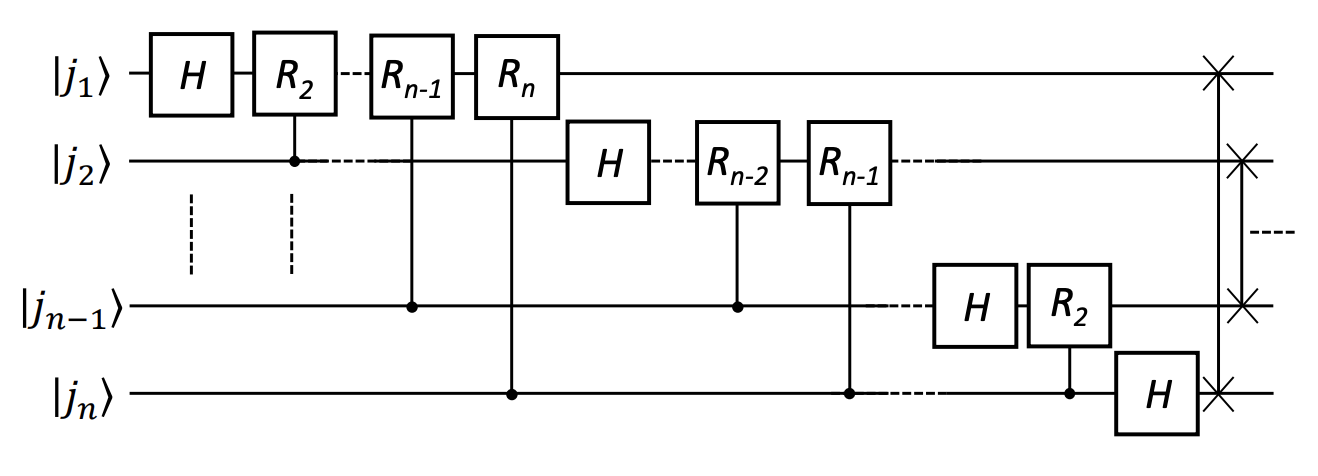
\includegraphics[scale=0.45]{img/qft.png}
\end{center}
Meanwhile, the qudit ($d=2^n$) clock and shift operators on $n$ qubits indexed by $\{q_j\}_{j=0}^{n-1}$ may be constructed as
\begin{align}
\T{Z}= \prod_{j=0}^{n-1} \T{R}_{q_j}(j+1) && \T{X}=\T{F}^\dagger \T{Z}\T{F}.
\end{align}
 Here $\T{R}_{q_j}$ denotes $\T{R}$ applied to the $q_j$'th qubit, and products ought to be understood from right to left. It is easiest to see that this works by direct calculation, e.g. for two qubits ($d=2^2=4$),
\begin{align}
\T{R}(1)\otimes \T{R}(2)
&= \begin{pmatrix} 1 & 0 \\ 0 & e^{\pi i }\end{pmatrix} \otimes   \begin{pmatrix} 1 & 0 \\ 0 & e^{\pi i/2}\end{pmatrix} 
	\\
&=\begin{pmatrix}1 & 0 & 0 & 0\\
0 &e^{\pi i /2} & 0 & 0 \\
0 & 0 & e^{\pi i } & 0 \\
0 & 0 & 0 & e^{3\pi i  /2} \end{pmatrix}\\
&=\sum_m e^{2\pi i m/4}|m\rangle\langle m|=\T{Z}.
\end{align}
Next, we need controlled counterparts of these operators. We first construct a qubit-controlled $\T{Z}$ operator,
\begin{align}
\T{QCZ}_{c,t} &= 	\prod_{j=0}^{n-1} \T{CR}_{c,t_j}(j+1),
\end{align}
which performs $\T{Z}$ on $n$ qubits indexed by $\{t_i\}_{i=1}^n$ conditional on the state of a control qubit $c$. For example, $\T{QCZ}$ on $1+3$ qubits:
\begin{center}
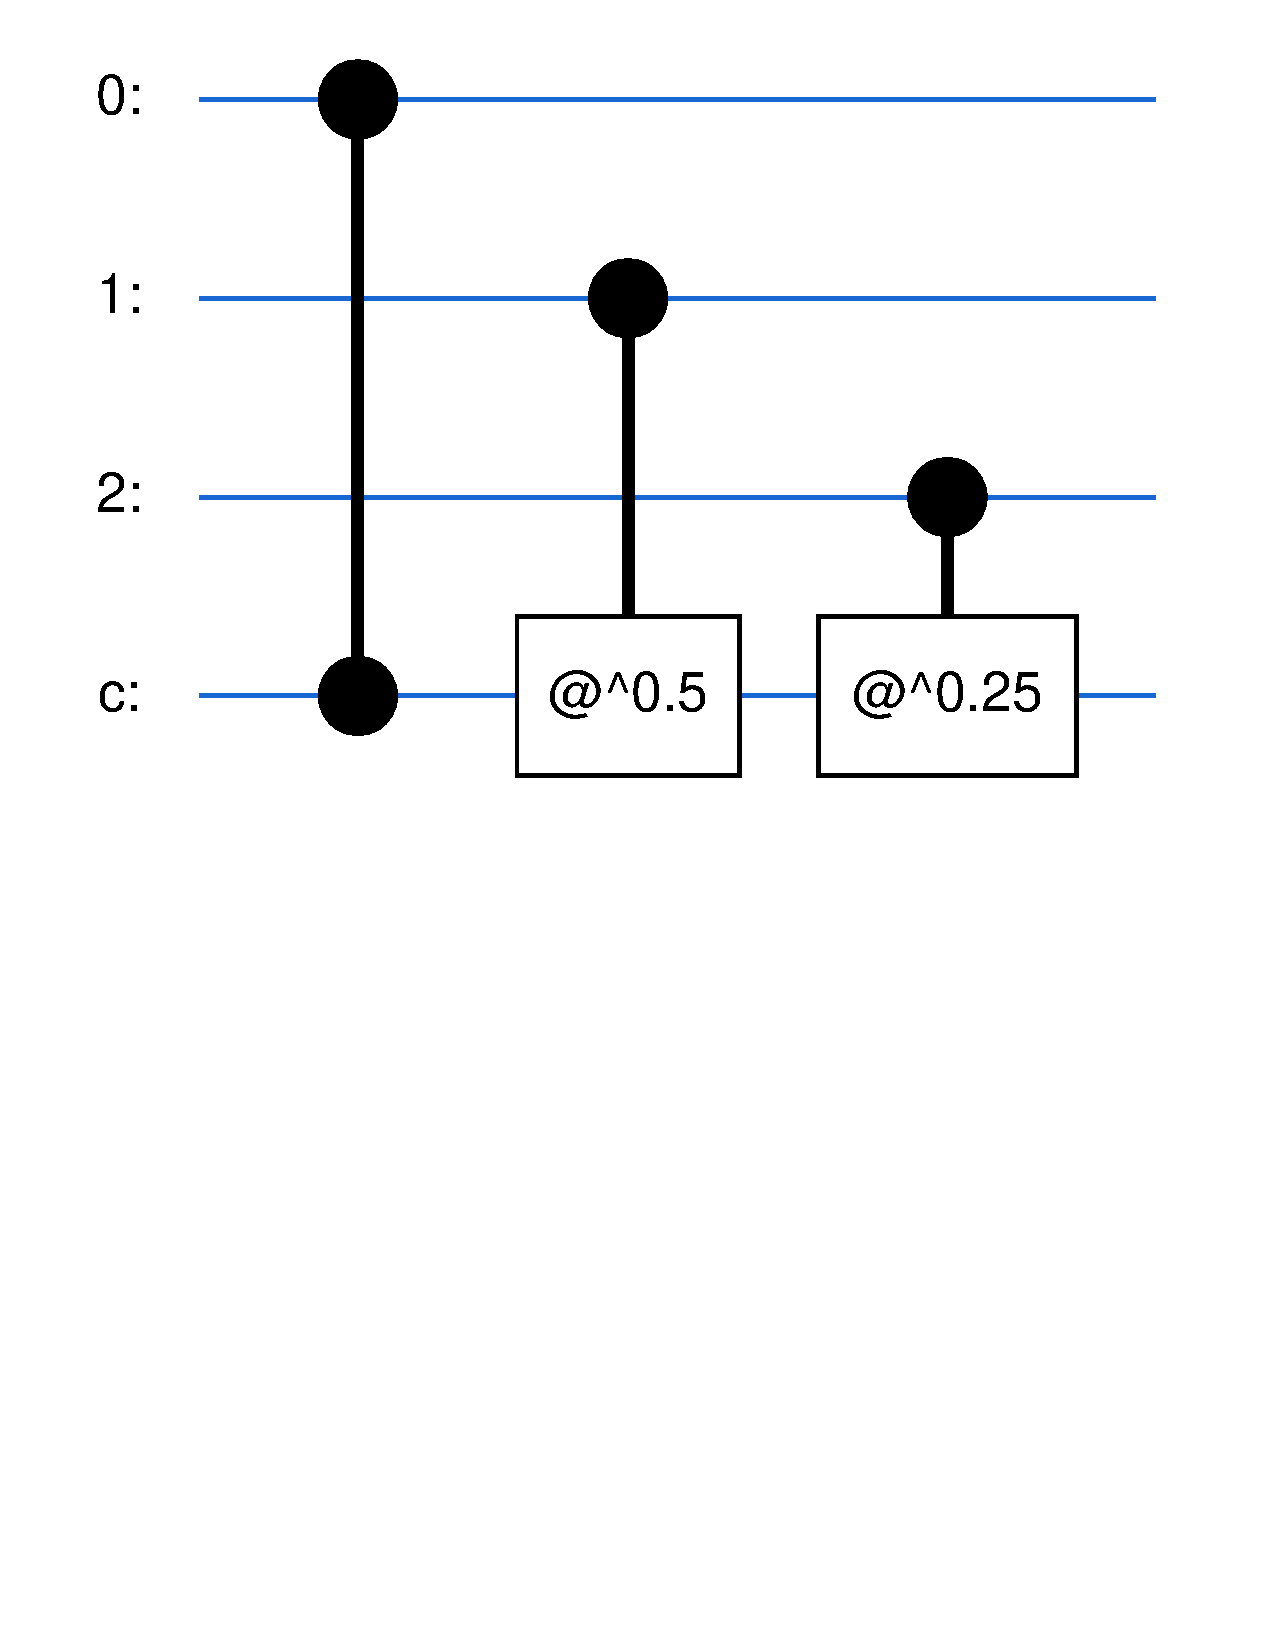
\includegraphics[scale=0.34]{img/qubit_controlled_clock.pdf}
\end{center}
The full qudit-controlled $\T{Z}$ operator, which performs $Z^k$ conditional on the control qudit being in the $|k\rangle$ state, may then be constructed as
\begin{align}
\T{CZ}_{c, t}	=\prod_{j=0}^{n-1} \T{QCZ}^{2^{j}}_{c_{n-j-1, t}},
\end{align}
where the control qudit is realized by $n$ qubits indexed by $\{c_j\}_{j=0}^{n-1}$, and the target qudit is realized by $n$  qubits indexed by $\{t_j\}_{j=0}^{n-1}$.  For example, $\T{CZ}$, where the first three qubits constitute the target qudit, and the second three qubits constitute the control:\begin{center}
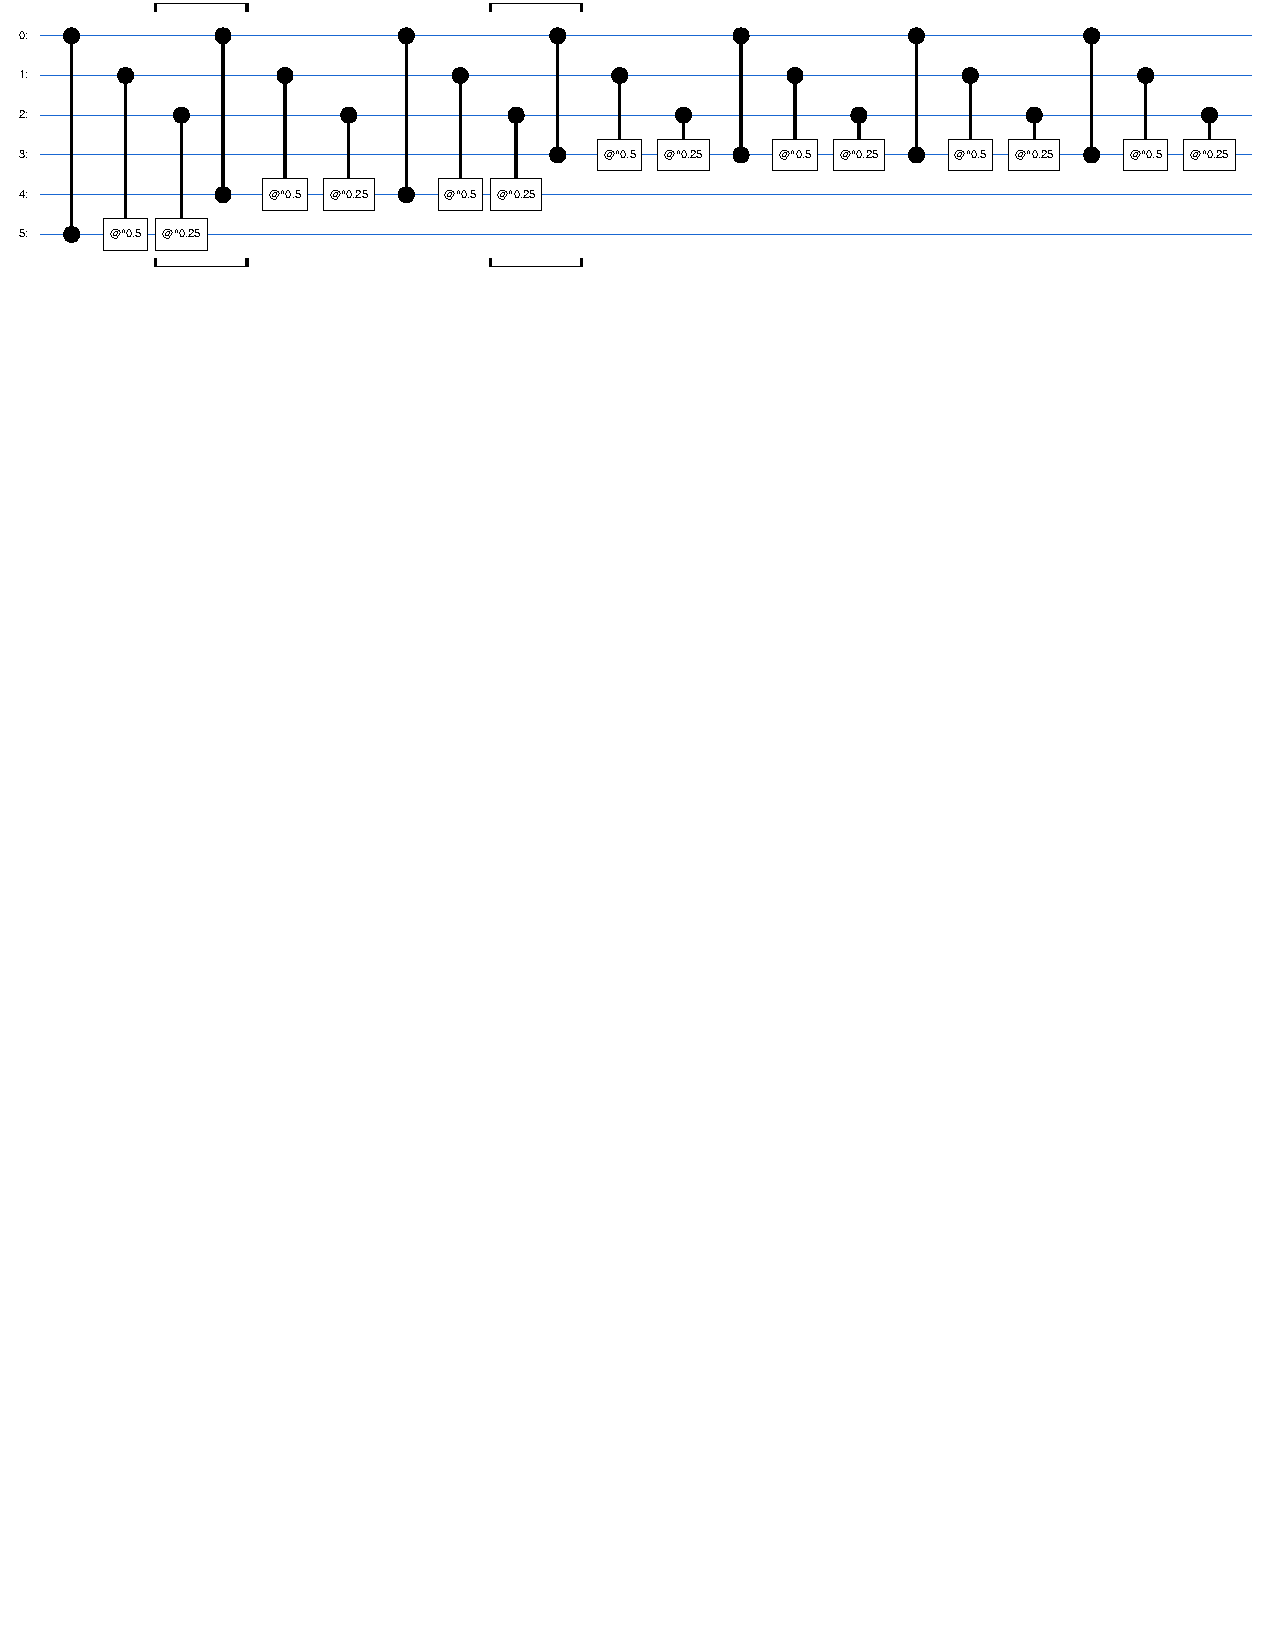
\includegraphics[scale=0.8]{img/controlled_clock.pdf}
\end{center}
Again, the logic is easiest to see by examining a simple case. Let $n=3$, and take the first three qubits to be the target, and the second three to be the control. Denoting $|0\rangle\langle 0| \equiv 0$ and $|1\rangle\langle 1 | \equiv 1$ and suppressing the tensor product sign, e.g. $ZII1=Z \otimes I \otimes I \otimes |1\rangle\langle 1| $, where the first tensor factor is a $2^3=8$ dimensional qudit, and the latter three tensor factors are treated as qubits,
\begin{align}
\T{CZ}_{c,t}&=\T{QCZ}^{2^2}_{0, t}\T{QCZ}^{2^1}_{1, t}\T{QCZ}^{2^0}_{2,t}\\
&=\Big(I0 II + Z^41II\Big)\Big(II0I+Z^2I1I\Big)\Big(III0+ZII1\Big) \\
&=\Big(I00I+Z^201I+Z^410I+Z^611I\Big)\Big(III0 + ZII 1\Big)\\
&=I000+Z001+Z^2010+Z^3011+Z^4100+Z^5101+Z^6110+Z^7111\\
&= \sum_{m=1}^{8}Z^m \otimes |m\rangle\langle m| .
\end{align}
Finally, $\T{CX}$ can be constructed by first applying $\T{F}$ to the target qubits, then $\T{CZ}$, followed by $\T{F}^\dagger$ on the target qubits. The Arthurs-Kelly unitary can then be expressed,
\begin{align}
\T{AK}= \T{F}_c\T{CX}_{c, t^{(2)}}  \T{F}^\dagger_c \T{CX}_{c,t^{(1)}}, 
\end{align}
where $c$ denotes the set of qubits realizing the qudit system of interest, and $t^{(1)}$ and $t^{(2)}$ are the two sets of qubits acting as ancillas. The first ancilla is shifted coherently conditional on the position of the system; then the second ancilla is shifted coherently conditional on the momentum of the system (hence the Fourier transforms). In circuit form, specializing the case that $n=2$, where the first qubit pair is ancilla 1, the second qubit pair is ancilla 2, and the third qubit pair is the system of interest, we have:
\begin{center}
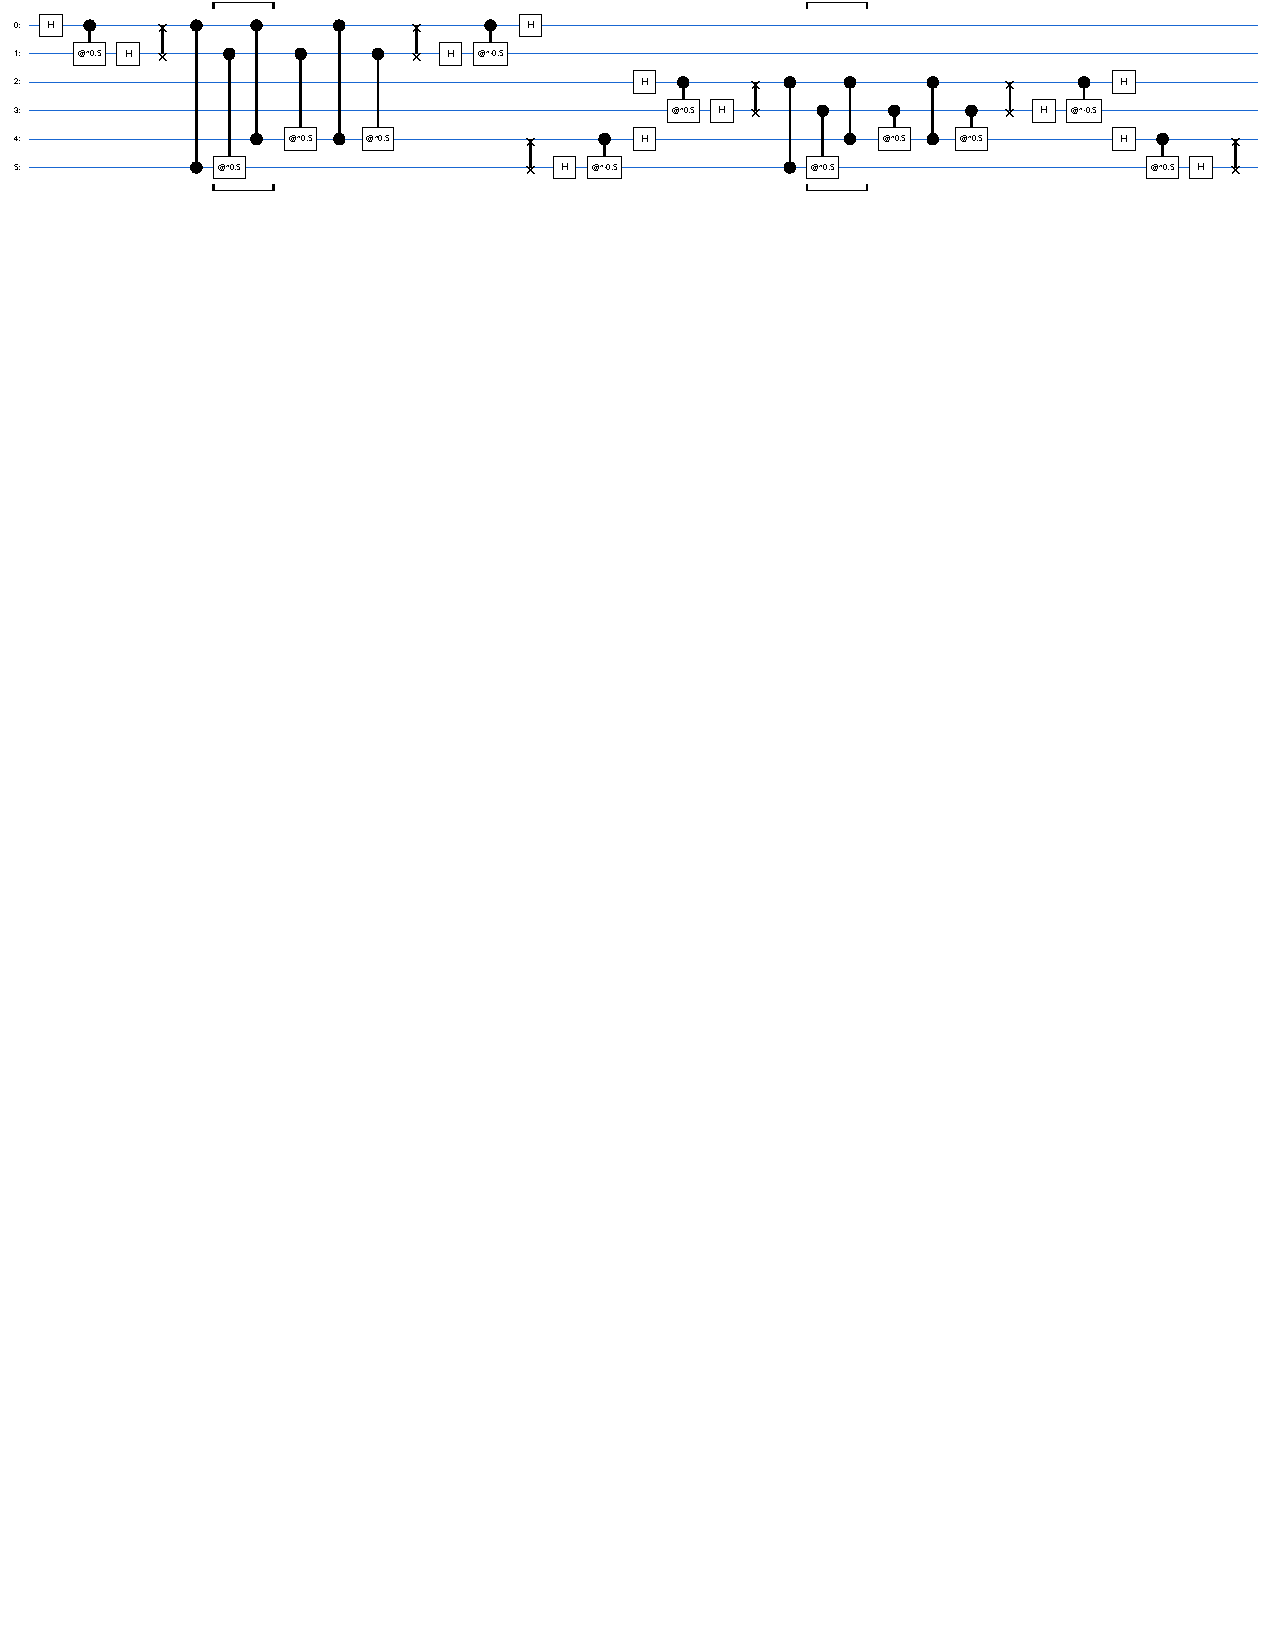
\includegraphics[scale=0.8]{img/ak.pdf}	
\end{center}
It then remains to prepare the initial state of the ancillas in order to realize the desired WH-POVM.


\section{Preparing ancillas for a $d=4$ SIC}

Following \cite{Scott_2010}, we will use the $4a$ fiducial whose components in the computational basis are 
\begin{align}
|\phi\rangle =  \frac{1}{\sqrt{\left(2-\sqrt{2}\right) \left(5+\sqrt{5}\right)}}\left(
\begin{array}{c}
  1
   \\
   \left(\frac{1}{8}+\frac{i}{
   8}\right)
   \left(\sqrt{2}+(-1-i)\right)
   \left(\left(1+\sqrt{5}\right)^{3/
   2}+(2-2
   i)\right)
   \\
i\left(\sqrt{2}-1\right)\\
   \left(\frac{1}{8}+\frac{i}{
   8}\right)
   \left(\sqrt{2}+(-1-i)\right)
   \left(\left(1+\sqrt{5}\right)^{3/
   2}+(-2+2
   i)\right)
\end{array}
\right)	.
\end{align}
By Eq. \!\ref{ancilla}, the corresponding ancilla state is 
\begin{align} |\gamma\rangle=\frac{1}{\left(2-\sqrt{2}\right) \left(5+\sqrt{5}\right)}
\left(
\begin{array}{c}
 \left(\frac{1}{8}+\frac{i}{8}\right)
   \left(\sqrt{2}+(-1-i)\right) \left((2+2
   i)+\sqrt{1+\sqrt{5}}+\sqrt{5
   \left(1+\sqrt{5}\right)}\right) \\
 1 \\
 \left(-\frac{1}{8}-\frac{i}{8}\right)
   \left(\sqrt{2}+(-1-i)\right) \left((-2-2
   i)+\sqrt{1+\sqrt{5}}+\sqrt{5
   \left(1+\sqrt{5}\right)}\right) \\
 -i \left(\sqrt{2}-1\right) \\
 -\frac{1}{2} \left(\sqrt{2}-2\right)
   \left(\sqrt{5}+(2-i)\right) \\
 \left(\frac{1}{8}+\frac{i}{8}\right)
   \left(\sqrt{2}+(-1+i)\right) \left((-2-2
   i)+\sqrt{1+\sqrt{5}}+\sqrt{5
   \left(1+\sqrt{5}\right)}\right) \\
 \left(\frac{1}{4}+\frac{i}{4}\right) \left(\sqrt{2}-2\right)
   \left((-3+i)-(1-i)
   \sqrt{5}+\left(1+\sqrt{5}\right)^{3/2}\right) \\
 \left(-\frac{1}{8}-\frac{i}{8}\right) \left((-1-3 i)+(1+2 i)
   \sqrt{2}\right) \left((-2-2 i)+\sqrt{1+\sqrt{5}}+\sqrt{5
   \left(1+\sqrt{5}\right)}\right) \\
 \frac{1}{2} \left((-3-i)+(2+i) \sqrt{2}\right) \left(-1+i
   \sqrt[4]{-9-4 \sqrt{5}}\right) \\
 i \left(\sqrt{2}-1\right) \\
 -\frac{1}{2} \left((-3-i)+(2+i) \sqrt{2}\right) \left(1+i
   \sqrt[4]{-9-4 \sqrt{5}}\right) \\
 3-2 \sqrt{2} \\
 \frac{1}{32} \left(\sqrt{2}+(-1-i)\right)
   \left(\sqrt{2}+(-1+i)\right) \left((2+2
   i)+\sqrt{1+\sqrt{5}}+\sqrt{5
   \left(1+\sqrt{5}\right)}\right)^2 \\
 \left(-\frac{1}{8}-\frac{i}{8}\right)
   \left(\sqrt{2}+(-1+i)\right) \left((2+2
   i)+\sqrt{1+\sqrt{5}}+\sqrt{5
   \left(1+\sqrt{5}\right)}\right) \\
 -\frac{1}{2} \left(\sqrt{2}-2\right)
   \left(\sqrt{5}+(2-i)\right) \\
 \left(\frac{1}{8}+\frac{i}{8}\right) \left((-1-3 i)+(1+2 i)
   \sqrt{2}\right) \left((2+2 i)+\sqrt{1+\sqrt{5}}+\sqrt{5
   \left(1+\sqrt{5}\right)}\right) \\
\end{array}
\right).\end{align}
It remains to be seen whether it is possible to construct an efficient preparation of this state, or whether one must string together an elaborate sequence of qubit $Z$ and $Y$ rotations interspersed with SWAP's to fit its $16-2=14$ parameters. One could hope that its \emph{algebraic number theoretic symmetries} lead to a clever method of preparation.

\bibliographystyle{plain} 
\bibliography{QuditArthursKelly}

\appendix 

\section{An alternative interpretation}
\label{alt-interpretation}

An interaction with Hamiltonian $A\otimes B$ can be interpreted in two different ways,
 \begin{align}
 	e^{i(A \otimes B)}=\sum_a|a\rangle\langle a| \otimes e^{iaB}=\sum_b e^{ibA}\otimes |b\rangle\langle b|,
 \end{align}
where $A=\sum_a a|a\rangle\langle a|$, $B=\sum_b b|b\rangle\langle b|$ are spectral decompositions. In other words, the very same interaction can be interpreted as controlled-$B$ operation, conditional on the observable $A$, or as a controlled $A$-operation, conditional on the observable $B$. In light of this, we may reconsider our Arthurs-Kelly interaction, rewriting it as
\begin{align}
U &= \left(\sum_m I \otimes X^m \otimes |m\rangle_p\langle m|_p	\right)\left(\sum_k X^k \otimes I \otimes |k\rangle\langle k|\right)\\
&=\left(\sum_m I \otimes e^{-imP} \otimes |m\rangle_p\langle m|_p	\right)\left(\sum_k e^{-ikP} \otimes I \otimes |k\rangle\langle k|\right)\\
&=e^{-i(I \otimes P \otimes P)}e^{-i(P \otimes I \otimes Q)}\\
&= \left(\sum_m I \otimes |m\rangle_p\langle m|_p\otimes e^{-imP} \right)\left(\sum_k |k\rangle_p\langle k|_p \otimes I \otimes e^{-ikQ}\right)	\\
&=\left(\sum_m I \otimes |m\rangle_p\langle m|_p\otimes X^m \right)\left(\sum_k |k\rangle_p\langle k|_p \otimes I \otimes Z^{-k}\right)\\
&=\sum_{km}|k\rangle_p\langle k|_p \otimes |m\rangle_p\langle m|_p \otimes X^mZ^{-k}\\
&=\sum_{km}|k\rangle_p\langle k|_p \otimes |m\rangle_p\langle m|_p \otimes D_{m,-k}.
\end{align}
From this point of view, the Arthurs-Kelly procedure involves coherently applying a WH displacement \emph{on the system} conditional on the momenta of two ancillas. The Kraus operators may be expressed
\begin{align}
K_{xy} &= \Big(\langle x, y| \otimes I\Big)U	\Big(|\gamma\rangle \otimes I\Big)\\
&=\sum_{km}\langle x|k\rangle_p \langle y|m\rangle_p \langle k, m|_p\gamma\rangle D_{m, -k}\\
&=\frac{1}{d}\sum_{km}\omega^{xk+ym}\langle k, m|_p\gamma\rangle D_{m, -k}.
\end{align}
As before, we consider
\begin{align}
K_{00}=	\frac{1}{d}\sum_{mk}\langle k,m|_p\gamma\rangle D_{m,-k},
\end{align}
and then examine $D_\B{a} K_{00} D_\B{a}^\dagger$. Since $D_\B{a}D_{m,-k}D_\B{a}^\dagger = 	\omega^{my+kx}D_{m,-k}$, we have
\begin{align}
	D_\B{a} K_{00} D_\B{a}^\dagger &= 	\frac{1}{d}\sum_{mk}\langle k,m|_p\gamma\rangle \omega^{xk+ym}D_{m,-k}=K_{xy},
\end{align}
which again shows that the measurement is WH-covariant. To find the initial state of the ancillas, we use the fact that the WH operators form a basis, so that we can identify
\begin{align}
	\langle k,m|_p\gamma\rangle =\frac{1}{\sqrt{d}}\tr(D_{m,-k}^\dagger \Pi),
\end{align}
or in the discrete position basis
\begin{align}
\langle k, m|\gamma\rangle = 	d^{-3/2}\sum_{ab} \omega^{am-bk}\tr(D_{a,b}^\dagger \Pi).
\end{align}

\section{A slight simplification}
\label{slight-simplification}
If we pull out Fourier transforms from the Arthurs-Kelly unitary
\begin{align}
U &= \left(\sum_m I \otimes X^m \otimes |m\rangle_p\langle m|_p	\right)\left(\sum_k X^k \otimes I \otimes |k\rangle\langle k|\right)\\
&=(I\otimes I\otimes F) \left(\sum_m I \otimes X^m \otimes |m\rangle\langle m|	\right)(I\otimes I \otimes F^\dagger)\left(\sum_k X^k \otimes I \otimes |k\rangle\langle k|\right),
\end{align}
we notice that strictly speaking we need not apply the final Fourier transform. Indeed, since this operation acts only on the system, and we are measuring the ancillas, applying the final $F$ ought not to affect our probability assignments for the outcomes of the measurement. If we drop the final Fourier transform, we obtain an alternative set of Kraus operators $\{K_{\B{a}}^\prime\}$ such that $E_\B{a}=K_\B{a}^\dagger K_\B{a}=K_\B{a}^{\prime \dagger} K_\B{a}^\prime$. While this simplifies the procedure, the resulting Kraus update is not a L\"uders update, and the post-measurement states will not be proportional to SIC states. This removes some of the conceptual simplicity of the sky-ground set-up beloved by QBists.

\end{document}